%!TEX root = ../thesis.tex

% Definitions:
%%%%%%%%%%%%%%
% Semantiv Web = samantisches Web

\chapter{Grundlagen} % (fold)
\label{cha:grundlagen}

%\todo[inline]{\Huge mehr QUELLEN!!!}

In diesem Kapitel werden einige grundlegende Begriffe und Techniken, die für das weitere Verständnis dieser Arbeit notwendig sind, behandelt. Zuerst werden zwei verbreitete Arten von Architekturen für den Zugriff auf Daten im World Wide Web (WWW, oder Web) gezeigt. Darauf folgt eine Einführung in das \emph{Sementic Web} und die Verwendung des \emph{Resource Description Frameworks} (RDF) und Ontologien für die Datenintegration von heterogenen Diskussionsplattformen im Web. Dabei werden die Ontologien des \emph{Friend of a Firend} (FOAF) und des \emph{Semantically-Interlinked Online Communities} (SIOC, ausgesprochen wie \enquote{Schock}) Projekts vorgestellt. Im Anschluss wird gezeigt, wie das \emph{Java Messaging Service} (JMS) Framework und die \emph{Enterprise Integration Patterns} (EIP) mit dem darauf aufbauenden Apache Camel für den Austausch von Daten über das Versenden und Empfangen von Nachrichten eingesetzt werden kann. Danach folgt eine kurze Beschreibung von fünf Lernplattformen und sozialen Online-Netzwerke, die später in der Implementierung eine Rolle spielen. Abschließend werden noch Projekte und Programme besprochen, die ein ähnliches Ziel wie das in dieser Arbeit vorgestellte System verfolgen.

\section{Zugriff auf Webanwendungen} % (fold)
\label{sec:zugriff_auf_webanwendungen}
%% korrigiert am 2013-10-01

Der Zugriff auf Daten von einer Webanwendung ist in den seltensten Fällen durch eine direkte Anbindung an die dahinter liegende Datenbank möglich beziehungsweise gewünscht. Gerade wenn das eigene Geschäft von diesen Daten abhängt, will man nur ungern alles mit allen teilen. Um trotzdem Dritten die Nutzung zu ermöglichen, kann anderen ein Zugriff über eine vordefinierte Programmierschnittstelle (API) gestattet werden. Für Anwendungen und Dienste im Web sind die folgenden zwei Ansätze für die Architektur einer solchen API sehr verbreitet. 

\subsection{Representational State Transfer (REST)} % (fold)
\label{sub:rest}
%% korrigiert am 2013-10-01

Eine sehr beliebte Architektur für den öffentlichen Zugriff auf Webanwendungen ist der \emph{Representational State Transfer} (REST). REST baut auf dem \emph{Hypertext Transfer Protocol} (HTTP) auf und definiert einige Beschränkungen die eine REST basierter Dienst erfüllen muss. 

Die Grundidee besteht darin, dass sich hinter einer Internetadresse eine bestimmte Ressource verbirgt, auf die man von außen zugreifen möchte. REST schreib aber nicht vor in welchem Datenformat diese Ressource übertragen werden soll, sondern es änderbar sein sollte. 

\begin{quote}
\enquote{REST components communicate by transferring a representation of a resource
in a format matching one of an evolving set of standard data types, selected dynamically
based on the capabilities or desires of the recipient and the nature of the resource.}\cite[S.\,87]{fielding2000architectural} 
\end{quote}

Dadurch wird einer einfachere Verwendbarkeit mit unterschiedliche Systemen ermöglicht. So kann für eine Webanwendung beim Aufrufen im Internetbrowser eine HTML-Datei zurück geliefert werden und falls ein Programm darauf zugreifen möchte, wird ein maschinenlesbares Format verwendet. Neben HTML sind auch noch XML und JSON sehr verbreitete Formate. Die Kommunikation wird dabei komplett Zustandslos abgehalten und alle Zustandsinformationen müssen immer mitgeliefert werden. Durch die Zustandslosigkeit skaliert das System viel besser, da Ressourcen sofort wieder frei gegeben werden können und nicht für spätere Anfragen gespeichert werden müssen.

Wie schon beschrieben, nutzen REST-basierte Dienste HTTP als Grundlage zur Kommunikation. Die dort definierten Operationen werden mit REST zur Auslieferung und Manipulation der Ressourcen verwendet. Zur Grundausstattung  gehören dabei \texttt{GET}, \texttt{POST}, \texttt{PUT} und \texttt{DELETE} (siehe Tabelle \ref{tbl:rest_oprations}). Die anderen Operationen \texttt{HEAD}, \texttt{TRACE}, \texttt{OPTIONS} und \texttt{CONNECT} sind eher selten anzutreffen (vgl. \cite[S.\,76ff]{fielding2000architectural}). 

\begin{table}[ht]
\centering
\caption{Wichtigsten HTTP Operationen mit REST} 
\begin{tabular}{r|p{12cm}}
    \textbf{Operation} & 
    \textbf{Beschreibung} \\ 
    \hline
    \texttt{GET} & 
    Liefert die hinter einer Adresse liegende Ressource an den Aufrufer zurück.\\
    
    \texttt{POST} & 
    Dient zum Anlegen einer neuen Ressource. Die URI der neuen Ressource ist beim Aufruf noch unbekannt und wird vom Service bestimmt. \\

    \texttt{PUT} & 
    Wird zum Ändern eine bestehenden Ressource genutzt. \\
    
    \texttt{DELETE} &
    Löscht, wie der Name schon sagt, eine Ressource.
\end{tabular}
\label{tbl:rest_oprations}
\end{table} 
     
% subsection rest (end)

\subsection{Simple Object Access Protocol (SOAP)} % (fold)
\label{sub:soap}
%% korrigiert am 2013-10-01

Das \emph{Simple Object Access Protocol} (SOAP) ist ein vom W3C standardisiertes Netzwerkprotokoll für den Austausch von Daten zwischen heterogenen Systemen. SOAP schreibt einen bestimmten Aufbau von Nachrichten vor, innerhalb derer die Daten transportiert werden. Als Repräsentation für diese Nachrichten wird hauptsächlich auf die Extensible Markup Language (XML)\footnote{\url{http://www.w3.org/XML}} gesetzt. Bei der Wahl des Transportprotokolls werden dahingegen keine Vorgaben gemacht und es ist frei wählbar. Häufig wird es aber in Verbindung mit HTTP und TCP verwendet. 

\begin{lstlisting}[
    language=XML,
    caption={SOAP Nachricht}\label{lst:soap_nachricht},
    captionpos=t]
<Envelope xmlns="http://www.w3.org/2003/05/soap-envelope">
    <Header>
        <!-- header information -->
    <Header> 
    <Body>
        <!--body content-->
    </Body>
</Envelope>
\end{lstlisting}

Eine Nachricht besteht im Grunde aus drei Elementen: den \emph{Envelope}, einen optionalen \emph{Header} und einem \emph{Body} (siehe Listing \ref{lst:soap_nachricht}). Der Envelope fungiert als Briefumschlag für die zu transportierenden Daten. Innerhalb jedes Envelopes können zusätzliche Meta-Informationen im Header Element gespeichert werden. Die eigentlichen Daten befinden sich im Body Element des Evelopes. Wie der Inhalt von Header und Body auszusehen haben wird von SOAP nicht vorgeschrieben. Dies können weitere XML Elemente oder einfache Zeichenketten sein (vgl. \cite{Mitra2007}). 

\subsubsection{Web Services Description Language} % (fold)
\label{ssub:wsdl}
%% korrigiert am 2013-10-01

% subsubsection wsdl (end)

Gebräuchlich ist der Einsatz von SOAP für \emph{Remote Procedure Calls} (RPC). Unter RPC verseht man den Aufruf eine Funktion von einem entfernten Dienst und das Zurückliefern einer eventuell vorhandenen Antwort. Welche Funktionen von einen Dienst zur Verfügung stehen, wird ein einer \emph{Web Services Description Language} (WSDL) Datei beschrieben. Diese WSDL-Datei wird im XML-Format verfasst und enthält alle wichtigen Informationen für RPC Aufrufe, die von einen Dienst zur Verfügung gestellt werden. Eine vollständige WSDL-Datei enthält dabei folgende Elemente:

\begin{description}
    \item[\textbf{types}:] Enthält Definitionen von Datentypen die in einer Message eingesetzt werden können. Zur Definition der Datentypen wird das Vokabular von \emph{XML Schema}\footnote{\url{http://www.w3.org/XML/Schema}} eingesetzt.
    \item[\textbf{message:}] Message-Elemente beschreiben den Aufbau der einzelnen Nachrichten.
    \item[\textbf{portType:}] Hier wird eine Menge an zur Verfügung stehenden Operationen definiert. Inklusive Eingabe- und Ausgabeparameter. In der WSDL Version 2.0 wurde portType in \emph{interface} umbenannt.
    \item[\textbf{binding}] beschreibt das Format und den Protokollablauf mehrerer Operationen. Zum Beispiel wie Eingabe- und Ausgabeparameter kodiert werden sollen. 
    \item[\textbf{port:}] Definiert eine Adresse hinter der sich ein Binding befindet. Üblicherweise in Form ein URI. Seit der WSDL Version 2.0 wird statt port der Begriff \emph{endpoint} verwendet.
    \item[\textbf{service}] Das Service-Element dient zum Zusammenfassen mehrerer Ports zu einen einzigen Dienst.
\end{description}

Wird eine solche WSDL-Datei öffentlich zugänglich gemacht, kann festgestellt werden welche Funktionen ein Dienst anbietet und automatisch APIs für unterschiedliche Systeme generiert werden. Der weiter Datenaustausch erfolgt dann über SOAP-Nachrichten (vgl. \cite{wsdl2001}).

% subsection wsdl_und_soap (end)

% section zugriff_auf_webanwendungen (end)

\section{Datenintegration} % (fold)
\label{sec:datenintegration}

Der Begriff Datenintegration beschreibt das zusammenführen von heterogenen Datenquellen an einen gemeinsamen Ort. Gerade bei der Integration verschiedener, teils kommerzieller Plattformen im Web ist dies ein Problem, da sie zwar ein ähnliches Ziel verfolgen aber sich von anderen abgrenzen wollen. So sind die verwendeten Datenformate in der Regel nicht direkt untereinander austauschbar. Um dies trotzdem zu erreichen, muss ein Mapping (Zuordnung) zwischen den verschiedenen Formaten erfolgen. In dieser Arbeit wird dazu auf RDF und Ontologien wie FOAF und SIOC gesetzt, welche im den Folgenden Abschnitten erklärt werden.

\subsection{Semantic Web} % (fold)
\label{sub:semantic_web}

Seit den Anfängen des Webs hat die Masse an abrufbaren Information immer weiter zugenommen, wobei die Vorteile des Webs eindeutig in der guten Aktualität und Erreichbarkeit von überall auf Erde liegen. Die Menge an Informationen sind aber auch ein Problem im Web. Da diese überall verteilt sind, ist es schwer für einen einzelnen alles zu einem Thema zu finden. Suchmaschinen wie Google\footnote{\url{https://www.google.com}}, Yahoo\footnote{\url{yahoo.com}} oder Microsoft Bing\footnote{\url{http://www.bing.com/}} leisten hier gute Dienste. Doch für Maschinen ist es noch immer nicht einfach die Inhalte von Webseiten zu verstehen, da diese für Menschen gemacht wurden. Auch das Erlernen von neuen Wissen anhand vorhandener Informationen ist in der aktuellen Form des Webs nur schwer realisierbar (vgl. \cite{Hitzler2008a}). 

2001 machte Tim Berners-Lee (der Erfinder des Webs) den Vorschlag das Web mit maschinenlesbaren Informationen zu erweitern und so die Verarbeitung mit Computerprogrammen zu vereinfachen (siehe \cite{Berners-Lee2001}). Die Idee des Semantic Webs wurde geboren. Der Inhalt des Webs wird mit semantischen Information so erweitert, dass Programme zum Beispiel erkennen können das zwei oder mehr Texte sich um das selbe Thema drehen ohne erst den Text analysieren zu müssen. Aber auch die Anzeige von impliziten Wissen wäre so einfacher möglich. Zum Beispiel sucht jemand eine Telefonnummer in Los Angeles, USA und will aus Deutschland anrufen. Anhand von zusätzlichen Informationen über die Länder erkennt das Programm, dass zwischen Los Angeles und Deutschland eine Zeitverschiebung von neun Stunden liegt. Es wird also vielleicht den Benutzer darüber informieren, erst am Nachmittag anzurufen, weil sein Gesprächspartner sonst noch schlafen würde.

\subsubsection{Resource Description Framework} % (fold)
\label{ssub:resource_description_framework}

Eine Baustein des Semantic Webs ist das Resource Description Framework. Wie der Name schon suggeriert, dient RDF zur Beschreibung von einzelnen Ressourcen innerhalb des Webs. Die Motivation bei der Entwicklung von RDF bestand darin, Information über Ressource in einem offenen Datenmodell zu speichern, so dass diese Daten von Maschinen automatisch verarbeitet, manipulieren und untereinander ausgetauscht werden können. Gleichzeitig sollte es auch einfach von jedem erweiterbar sein. Ressourcen stellen dabei alle Dinge dar, über die man eine Aussage treffen kann (vlg. \cite{Klyne2004,Manola2004}). 

\begin{quote}
\enquote{RDF is designed to represent information in a minimally constraining, flexible way.}\cite[Abschnitt 2.1 \enquote{Motivation}]{Klyne2004}
\end{quote}

Das Datenmodell von RDF ist zur effizienten Verarbeitung sehr einfach aufgebaut. Die Grundlage bilden Tripel (Eine Menge von genau 3 Elementen) aus Subjekt, Prädikat und Objekt. Eine oder mehrere solcher Triple zusammen werden als gerichteter RDF-Graph bezeichnet. Subjekt und Objekt stehen über das Prädikat mit einander in Beziehung, wobei die Beziehung immer vom Subjekt zum Objekt geht. Das Prädikat wird auch als Eigenschaft (engl. Property) bezeichnet. Gemeinsam beschreibt das Triple immer eine Aussage über eine oder zwei Ressourcen. Zum Beispiel \enquote{Die Dose enthält Kekse} wäre eine Aussage, dass in der Ressource Dose sich andere Ressourcen und zwar Kekse befinden. Die \enquote{Dose} ist dabei das Subjekt, \enquote{enthält} das Prädikat und \enquote{Kekse} das Objekt. Ein Triple ist quasi ein einfacher Satz in der natürlichen Sprache. Für die Belegung von Subjekt, Prädikat und Objekt mit Werten werden in RDF \emph{Uniform Resource Identifier} (URI), \emph{Literale} oder \emph{leere Knoten} (im Englischen \emph{Blank Nodes} genannt) verwendet. 

\begin{description}
    \item[\textbf{URIs}] sind eindeutige Bezeichner, die eine beliebige reale oder abstrakte Ressource darstellen und werden wie im \emph{RFC 2396}\footnote{\url{http://www.isi.edu/in-notes/rfc2396.txt}} beschrieben formatiert. Relative URIs sollten aber nach \cite{Klyne2004} möglichst vermieden werden. URIs bilden eine Verallgemeinerung der im Web gebräuchlichen Uniform Resource Locator (URL). Diese Arbeit verwendet aber auch für URLs einheitlich den Begriff URI.
   
    \item[\textbf{Literale}] bestehen aus einfachen Zeichenketten die zum Speichern der Informationen dienen. Zusätzlich können Literale mit der Angabe der verwendeten Sprache \texttt{"{}Objekt"{}@de} oder des Datentyps \texttt{"{}42"{}\^{}\^{}xsd:integer} erweitert werden. Bei Literalen ist darauf zu achten, dass die Literale \texttt{"{}Objekt"{}}, \texttt{"{}Objekt"{}@de} und \texttt{"{}Objekt"{}\^{}\^{}xsd:string} auf den ersten Blick zwar den selben Wert beschreiben, aber aus Sicht von RDF nicht die selben sind. Sowohl die angegebene Spracht als auch der Datentyp müssen übereinstimmen, um zwei Literale als gleich anzuerkennen.

    \item[\textbf{Leere} Knoten] werden als alle Knoten im RDF Graphen beschrieben, welche weder eine URI noch ein Literal sind. Sie dienen häufig dazu, um Subjekte zu beschreiben für die nicht unbedingt eine eigene URI nötig ist. Leere Knoten sind nur innerhalb eines Graphen eindeutig, weshalb sie für Referenzierungen von Ressourcen außerhalb des RDF-Graphen ungeeignet sind.
\end{description}

Doch nicht jede dieser drei Belegungen ist in jedem Teil des Tripels erlaubt. Das Subjekt ist entweder eine URI oder ein leerer Knoten, wobei das Prädikat nur eine URI sein kann. Dahingegen ist es beim Objekt möglich eine URI, einen leeren Knoten oder ein Literal zu verwendeten. 

% subsubsection resource_description_framework (end)

\subsubsection{Repräsentation von RDF-Graphen} % (fold)
\label{ssub:darstellung_von_rdf_graphen}

In Laufe der Zeit von RDF wurde verschiedene Möglichkeiten erfunden einen RDF-Graphen darzustellen. In diesem Abschnitt werden drei Formen vorgestellt, die auch in dieser Arbeit zur Visualisierung benutzt werden. Zuerst die graphische Darstellung für das visualisieren von RDF-Daten in Abbildungen, dann eine Form mit XML und als letztes die platzsparenden Sprache Turtle.

\paragraph{Graphische Darstellung} % (fold)
\label{par:graphische_darstellung}

Graphisch lässt sich RDF als gerichteter Graph mit Knoten und Kanten darstellen. Ressourcen werden dabei als Ellipsen, Literale als Rechtecke und die Prädikate als gerichtete Kante dazwischen gezeichnet. Ein Beispiel ist in Abbildung \ref{fig:graphisch_rdf_triple} zu sehen. Es verdeutlicht noch einmal den Aufbau von RDF-Dokumenten als gerichteter Graph.

    \begin{figure}[ht]
        \centering
        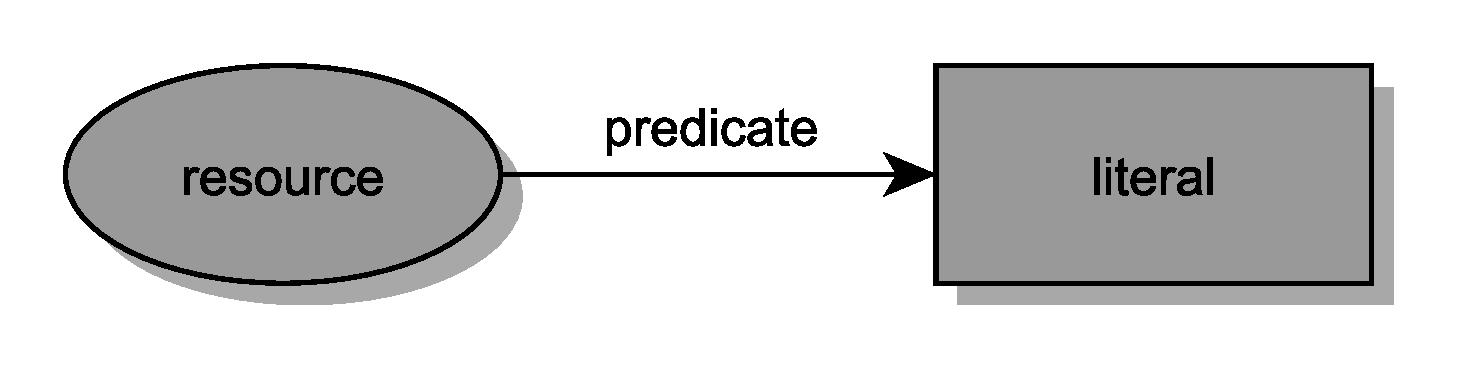
\includegraphics[
            width=0.6\textwidth,
            keepaspectratio=true,
            clip=true]
            {assets/images/rdf-triple}
        \caption{Einfacher RDF-Graph}
        \label{fig:graphisch_rdf_triple}
    \end{figure}

% paragraph graphische_darstellung (end)

\paragraph{RDF/XML} % (fold)
\label{par:rdf_xml}

RDF/XML ist eine verbreitete Form RDF-Dokumente zu beschreiben. Die Basis bildet hierbei die Verwendung von XML. In Listing \ref{lst:rdf_xml_beispiel} ist ein Beispieldokument in RDF/XML zusehen. Das in Zeile 2 zu sehende \texttt{rdf:RDF} ist das Wurzelelement für den RDF-Graphen. In diesem Wurzelelement werden mit \texttt{xmlns:\dots} einige Präfixe für Namensräume  definiert, um das Dokument übersichtlicher zu gestalten. Alle Präfixe werden danach mit den angegebenen Namensraum ersetzt. Das \texttt{Description}-Element in Zeile 5 stellt die Beschreibung einer Ressource im RDF-Graphen dar. Die URI der Ressource wird mit dem Attribut \texttt{rdf:about} definiert. Innerhalb des Description-Elements befinden sich die Prädikate. In Zeile 6 steht also, dass die Ressource die Eigenschaft \texttt{exterms:enthaelt} hat und auf das Literal \texttt{Kekse} verweist. Wäre das Objekt nicht wie hier ein Literal sondern eine weitere Ressource, könnte man über das Attribut \texttt{rdf:ressource} für das Element \texttt{exterms:enthaelt} die URI der Ressource angeben.

\begin{lstlisting}[
    language=XML,
    caption={RDF/XML Beispiel}\label{lst:rdf_xml_beispiel},
    captionpos=t]
<?xml version="1.0"?>
<rdf:RDF xmlns:rdf="http://www.w3.org/1999/02/22-rdf-syntax-ns#"
    xmlns:exterms="http://www.example.org/terms#">

    <rdf:Description rdf:about="http://www.example.org/dose">
       <exterms:enthaelt>Kekse</exterms:enthaelt>
    </rdf:Description>
</rdf:RDF>
\end{lstlisting}
% paragraph rdf_xml (end)

\paragraph{Turtle} % (fold)
\label{par:turtle}

Turtle (Ausgeschrieben: \emph{Terse RDF Triple Language}) ist eine weiter Möglichkeit RDF-Graphen darzustellen und ging aus der Sprache N3\footnote{\url{http://www.w3.org/DesignIssues/Notation3.html}} (Kurzform für Notation 3) hervor (siehe. \cite{DavidBeckett}). In Turtle wird das Triple aus Subjekt, Prädikat und Objekt hintereinander geschrieben und zwischen jeden mindestens ein Leerzeichen gelassen. Als Abschluss folgt nach jedem Tripel noch ein Punkt. Der Punkt verdeutlicht noch einmal die Ähnlichkeit mit gesprochenen Sätzen. Listing \ref{lst:turtle_beispiel} zeigt das Beispiel mit der Keksdose noch einmal in Turtle Notation. 

\begin{lstlisting}[
    caption={Turtle Beispiel}\label{lst:turtle_beispiel},
    captionpos=t]
<http://www.example.org/dose> <http://www.example.org/terms#enthaelt> "Kekse" .
\end{lstlisting} 


In Turtle ist darauf zu achten, dass alle URIs immer zwischen spitzen Klammern stehen müssen und Literale werden in Anführungszeichen geschrieben. Da nun einzelne Prädikate beziehungsweise allgemein URIs recht häufig innerhalb eines Graphen auftauchen können, kann es einfacher sein diese abzukürzen. Wie schon in RDF/XML können auch in Turtle Präfixe definiert werden, um Schreibarbeit zu sparen und den RDF-Graphen für Menschen lesbarer zu gestalten.

\begin{lstlisting}[
    caption={Turtle Präfixe}\label{lst:turtle_prefix},
    captionpos=t]
@prefix exterms: <http://www.example.org/terms#> .
<http://www.example.org/dose> exterms:enthaelt "Kekse" .   
\end{lstlisting}

In der ersten Zeile von Listing \ref{lst:turtle_prefix} wird durch Einleiten mit dem Schlüsselwort \texttt{@prefix} ein neuer Präfix \texttt{exterms:} für den Namensraum \texttt{http://www.example.org/terms\#} festgelegt. Dieser Präfix kann nun überall innerhalb des Dokumentes verwendet werden, wobei die spitzen Klammern dann weggelassen werden können.

\begin{lstlisting}[
    caption={Turtle abkürzende Schreibweise}\label{lst:turtle_shortcut},
    captionpos=t]
@prefix exterms: <http://www.example.org/terms#> .
<http://www.example.org/dose> exterms:farbe "blau";
    exterms:enthaelt "Kekse", "Geld" .   
\end{lstlisting}

Listing \ref{lst:turtle_shortcut} zeigt ein drittes Beispiel, wie redundante Angaben eingespart werden können. Wie man in der zweiten Zeile sehen kann, wird das Triple mit einem Semikolon abschlossen und nicht mit einen Punk. Durch das Semikolon ist es Möglich das Subjekt mehrfach wiederzuverwenden, wenn sich nur Prädikat und Objekt ändern. So können sich mehrere Eigenschaften einer Ressource platzsparend schreiben lassen ohne das Subjekt immer wieder anzugeben. Ändert sich dahingegen nur das Objekt, können mehrere durch Kommata getrennt hintereinander geschrieben werden. Die dritte Zeile beschreibt zum Beispiel, dass in der Dose nicht nur Kekse sonder auch Geld steckt. 

Leere Knoten können dann noch in Turtle durch angeben einer geöffneten eckigen Klammer gefolgt von einer sich schließenden dargestellt \enquote{\texttt{[]}}. Zwischen diesen beiden Klammern kann zusätzlich eine Menge von Prädikaten und ihren Objekten stehen, die von Semikolons getrennt werden. Beispiele dazu sind im Anhang \ref{sec:anhang_proof_of_concept_konfigurationsdaten} zu sehen. Soll ein leerer Knoten innerhalb eines Graphen referenziert werden, kann er auch als \texttt{\_:LABEL}, wobei \texttt{LABEL} ein beliebiger Beizeichner ist, geschrieben werden.

% paragraph turtle (end)

% subsubsection darstellung_von_rdf (end)

% subsection semantic_web_und_das_resource_description_framework (end)

\subsection{Ontologien} % (fold)
\label{sub:ontologien}

Sollen Daten aus verschiedenen Quellen zusammengefügt werden, stellt sich häufig das Problem dass Teile dieser dieser Daten zwar den gleichen Sinn haben, aber aufgrund der Sichtweise des jeweiligen Systems eine andere Bezeichnung besitzen. Dies kann zum Beispiel zu Missverständnissen bei der Verarbeitung führen oder dass Teile eines anderen Systems nicht wiederverwendet werden können \cite[S.\,13]{Uschold1996a}. Einen Ausweg aus diesem Dilemma kann die Verwendung von Ontologien zeigen. Ontolgien können allgemein als Wissensbasis \cite[S.\,2]{Uschold1996a}\cite[S.\,12]{Hitzler2008a} bezeichnet werden und liefern eine formale Spezifikation über eine bestimmte Interessensdömäne. Sie beschreibt nicht nur wie das verwendete Vokabular aussieht, sondern legt auch fest welche einheitliche Bedeutung jede Vokabel hat. 

Im Bereich des Semantic Webs sind heutzutage zwei Sprachen für die Erstellung von Ontologien verbreitet. Diese sind \emph{RDF Schema} (RDFS)\cite{Brickley} und die darauf aufbauende \emph{Web Ontology Language} (OWL)\cite{partelschneider2004}. Beide Sprachen basieren auf RDF, so können sie zusammen mit jedem System verwendet werden, das RDF versteht. Mit ihnen ist man im Stande abstrakte Klassen von Dingen und deren Eigenschaften zu definieren und diese in eine Vererbungshierarchie einzugliedern. Die Ausprägung eine Klasse wird als Individuum bezeichnet, in dieser Arbeit wird aber Begriff Objekt aus der objektorientierten Programmierung verwendet, um die Überleitung von der theoretischen Beschreibung zu Implementierung einheitlich zu halten. Im Gegensatz zu RDFS können in OWL diverse Einschränkungen definiert werden. Wie zum Beispiel, dass eine Eigenschaft nur einmal pro Objekt einer Klasse vorhanden sein darf. Die Anhänge \ref{sec:anhang_socc_connector_config_ontologie} und \ref{sec:anhang_sioc_services_authentication_module} zeigen zwei Ontologien in der Sprache OWL, welche innerhalb dieser Arbeit entwickelt wurden und in Abschnitt \ref{sub:connector_config_ontologie} und \ref{sub:authentifizierung} beschreiben werden.

\subsubsection{Friend of a Friend (FOAF)} % (fold)
\label{ssub:friend_of_a_friend_}

Friend of a Friend\footnote{\url{http://www.foaf-project.org}} ist ein im Jahr 2000 gestartetes Projekt, das versucht Personen innerhalb des Webs, inklusive der Verbindungen zwischen ihnen und anderen, sowie dem was sie machen, in maschinenlesbarer Form abzubilden. FOAF stellt hierzu eine Ontologie \cite{Brickley2010} (RDF-Präfix \texttt{foaf:}) für solche sozialen Netzwerke zur Verfügung. Das Vokabular von FOAF gliedert sich dazu in einen \enquote{FOAF Core} und einen \enquote{Social Web} Bereich. Der Core-Bereich enthält die Klasse \texttt{foaf:Agent} für alle Dinge die eine Handlung ausführen können. Also sowohl natürliche Personen, Gruppen oder Organisationen, als auch Computerprogramme oder Maschinen. Für diese gibt es jeweils noch einzelne Unterklassen die von der Klasse \texttt{foaf:Agent} erben. Objekten dieser Klassen können eigene Eigenschaften wie einen Namen, ein Alter oder wen sie kennen, gegeben werden. Der Sozial Web Bereich enthält alle Teile die für das Web interessant sind. Das wären zum Beispiel welche E-Mail-Adresse eine Person besitzt, welche Benutzerkonten ihm auf welcher Webseite gehören oder wie die URI seiner Homepage lautet. Das FOAF Projekt sieht sich aber selber nicht als Konkurrenz gegenüber den etablierten sozialen Online-Netzwerken, sondern eher ein Ansatz für einen besser Austausch zwischen den einzelnen Seiten \cite[siehe \enquote{Abstract}]{Brickley2010}.

Listing \ref{lst:foaf_beispiel} zeigt ein Beispiel für ein FOAF-Dokument in RDF/XML. Es beschreibt die fiktive Person \enquote{Max Hiwi}, mit Vor- und Nachname sowie der Hashwert seiner E-Email-Adresse (\texttt{foaf:mbox\_sha1sum}). Diese Person kennt (\texttt{foaf:knows}) eine Person mit dem Namen \enquote{John Doe} der ebenso eine E-Mail-Adresse mit den angegeben Hashwert besitzt. Statt die Eigenschaften von John Doe hier noch einmal vollständig anzugeben, wird über die Eigenschaft \texttt{rdfs:seeAlso} auf ein weiteres FOAF-Dokument verwiesen, dass die fehlenden Daten enthält. 

\begin{lstlisting}[
    language=XML,
    caption={FOAF Beispiel}\label{lst:foaf_beispiel},
    captionpos=t]
<rdf:RDF xmlns:rdf="http://www.w3.org/1999/02/22-rdf-syntax-ns#"
         xmlns:rdfs="http://www.w3.org/2000/01/rdf-schema#"
         xmlns:foaf="http://xmlns.com/foaf/0.1/">
  <foaf:Person>
    <foaf:name>Max Hiwi</foaf:name>
    <foaf:firstName>Max</foaf:firstName>
    <foaf:surname>Hiwi</foaf:surname>
    <foaf:mbox_sha1sum>dce4fc922158f8b26fbf0a65ea32bfab58488bd2</foaf:mbox_sha1sum>
    <foaf:knows>
      <foaf:Person>
        <foaf:name>John Doe</foaf:name>
        <foaf:mbox_sha1sum>479ea35d3522662b70dc7afd721853485c95db57</foaf:mbox_sha1sum>
        <rdfs:seeAlso rdf:resource="http://www.example.org/people/jd/foaf.rdf"/>
      </foaf:Person>
    </foaf:knows>
  </foaf:Person>
</rdf:RDF>
\end{lstlisting}

% subsubsection friend_of_a_friend_ (end)

\subsubsection{Semantically-Interlinked Online Communities (SIOC)} % (fold)
\label{ssub:semantically_interlinked_online_communities}

Semantically-Interlinked Online Communities ist ein Projekt, welches von Uldis Boj\=ars und John Breslin begonnen wurde, um unterschiedliche, webbasierte Diskussionsplattformen(Blog, Forum, Mailinglisten,\dots) untereinander verbinden zu können (siehe \cite{Breslin2005,Bojars2008a}). Der Kern von SIOC besteht aus einer Ontologie\cite{deri2013} (RDF-Präfix \texttt{sioc:}), welche den Inhalt und die Struktur dieser Plattformen in ein maschinenlesbares Format bringen kann und es erlaubt diese auf semantischer Ebene zu verbinden. Auch sollte es möglich sein Daten von einer Plattform zu einer Anderen zu transferieren und so einfacher Inhalte austauschen zu können. Als Basis für SIOC dient RDF, die Ontologie selber wurde in RDFS und OWL umgesetzt. Um nicht das Rad neu erfinden zu müssen, greift SIOC auf schon bestehende und bewährte Ontologien zurück. Für die Abbildung von Beziehungen zwischen einzelnen Personen wird FOAF und für einige Inhaltliche- und Metadaten (Titel, Inhalt, Erstelldatum, \dots) Dublin Core Terms\footnote{\url{http://dublincore.org/documents/dcmi-terms}} eingesetzt.

\begin{figure}[ht]
    \centering
    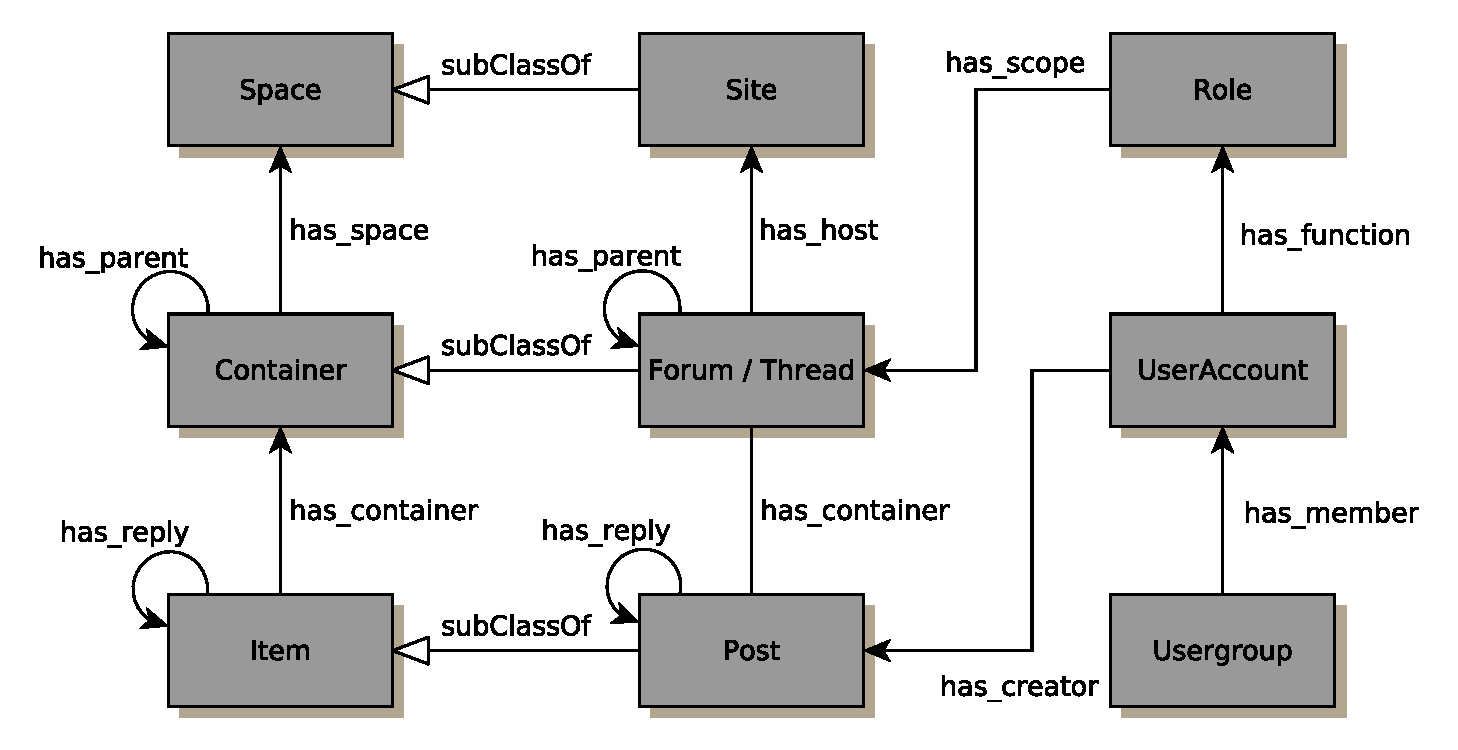
\includegraphics[
        width=\textwidth,
        keepaspectratio=true,
        clip=true]
        {assets/images/sioc_overview}
    \caption{Aufbau von SIOC (modifiziert) - Originalquelle: \cite{deri2013}}
    \label{fig:sioc_aufbau_diagramm}
\end{figure}

Die wichtigsten Klassen von SIOC sind in Abbildung \ref{fig:sioc_aufbau_diagramm} zu sehen. Die Klasse \texttt{sioc:Site} ist für die Beschreibung von Webseiten, in denen Beiträge innerhalb von Containern verfasst werden. Ein solcher Container ist die Klasse \texttt{sioc:Forum} und steht für einen Ort an dem Beiträge geschrieben werden. Enthält ein Forum Diskussionen zu unterschiedlichen Themen, kann es noch einmal mit der Klasse \texttt{sioc:Thread} unterteilt werden, welche immer ein Forum als Elternteil haben müssen (\texttt{sioc:has\_parent}). Beide Klassen leiten sich von der Klasse \texttt{sioc:Container}, als einen allgemeinen Ort für Beiträge, ab. Die einzelnen Beiträge werden durch die Klasse \texttt{sioc:Post} beziehungsweise von der übergeordneten Klasse \texttt{sioc:Item} modelliert. Beiträge gehören in der Regel immer zu einen bestimmten Container oder mindesten zu einer Webseite. Es ist auch mögliche Beiträge als Kommentar zu anderen Beiträgen über die Eigenschaft \texttt{sioc:has\_reply} abzubilden (vgl. \cite[S.\,203ff]{Breslin2009}). Jeder Beitrag besitzt mindesten einen Autor der ein Benutzerkonto auf der betreffenden Seite besitzt. Für die Beschreibung eines solchen Benutzerkontos wird die Klasse \texttt{sioc:UserAccount} verwendet. Dieses Benutzerkonto kann zusätzlich zu einer Gruppe gehören. Über die Klasse \texttt{sioc:Role} kann einen Benutzerkonto eine bestimmte Rolle innerhalb einer Webseite, Forum und so weiter zugeteilt werden. Ein Beispiel dafür wäre die Rolle eines Moderator, der überwacht ob die Regel der Seite in den einzelnen Foren eingehalten werden.

% subsubsection semantically_interlinked_online_communities (end)

% subsection ontologien (end)

% section datenintegration (end)

\section{Datenaustausch} % (fold)
\label{sec:datenverteilung}

Sollen zwischen zwei unabhängigen Systemen Daten ausgetauscht werden, hat man im Allgemeinen mehrere Ansätze dieses Problem zu lösen. Beide Programme könnten Dateien mit den Daten an einen festen Ort speichern, die der jeweilig andere lesen kann. Auch ist das Benutzen eines gemeinsamen Datenbankmanagementsystems oder die Verwendung von RPCs denkbar. Ebenso ist der Datenaustausch mit Nachrichten über ein Netzwerk ein sehr flexibler und sicherer Weg. Jeder dieser Ansätze hat seine eigenen Vor- und Nachteile und sollte am Besten nach den Anforderungen für den Verwendungszweck gewählt werden (vgl. \cite[S.\,12]{Hohpe:2003:EIP:940308}). 

Dieser Abschnitt beschäftigt sich explizit nur mit dem Versenden und Empfangen von Nachrichten, da dies für das in der Einleitung beschriebene Wunschsystem die meisten Vorteile bringt. Dazu wird zuerst das \emph{Java Messageing Service}-Framework (JMS) vorgestellt und danach die Enterprise Integration Patterns (EIP) mit Apache Camel.

%\todo[inline]{Datenverteilung-Einleitung schreiben}

\subsection{Java Messaging Service} % (fold)
\label{sub:java_messaging_service}

JMS \cite{jms} ist ein Sammlung von Schnittstellen für das Erstellen, Senden und Empfangen von Nachrichten zwischen Programmen in Java. JMS erlaubt eine Entwicklung von verteilten Anwendung, die nicht nur lose gekoppelt, sondern auch asynchron und zuverlässig arbeiten. 

\begin{figure}[ht]
    \centering
    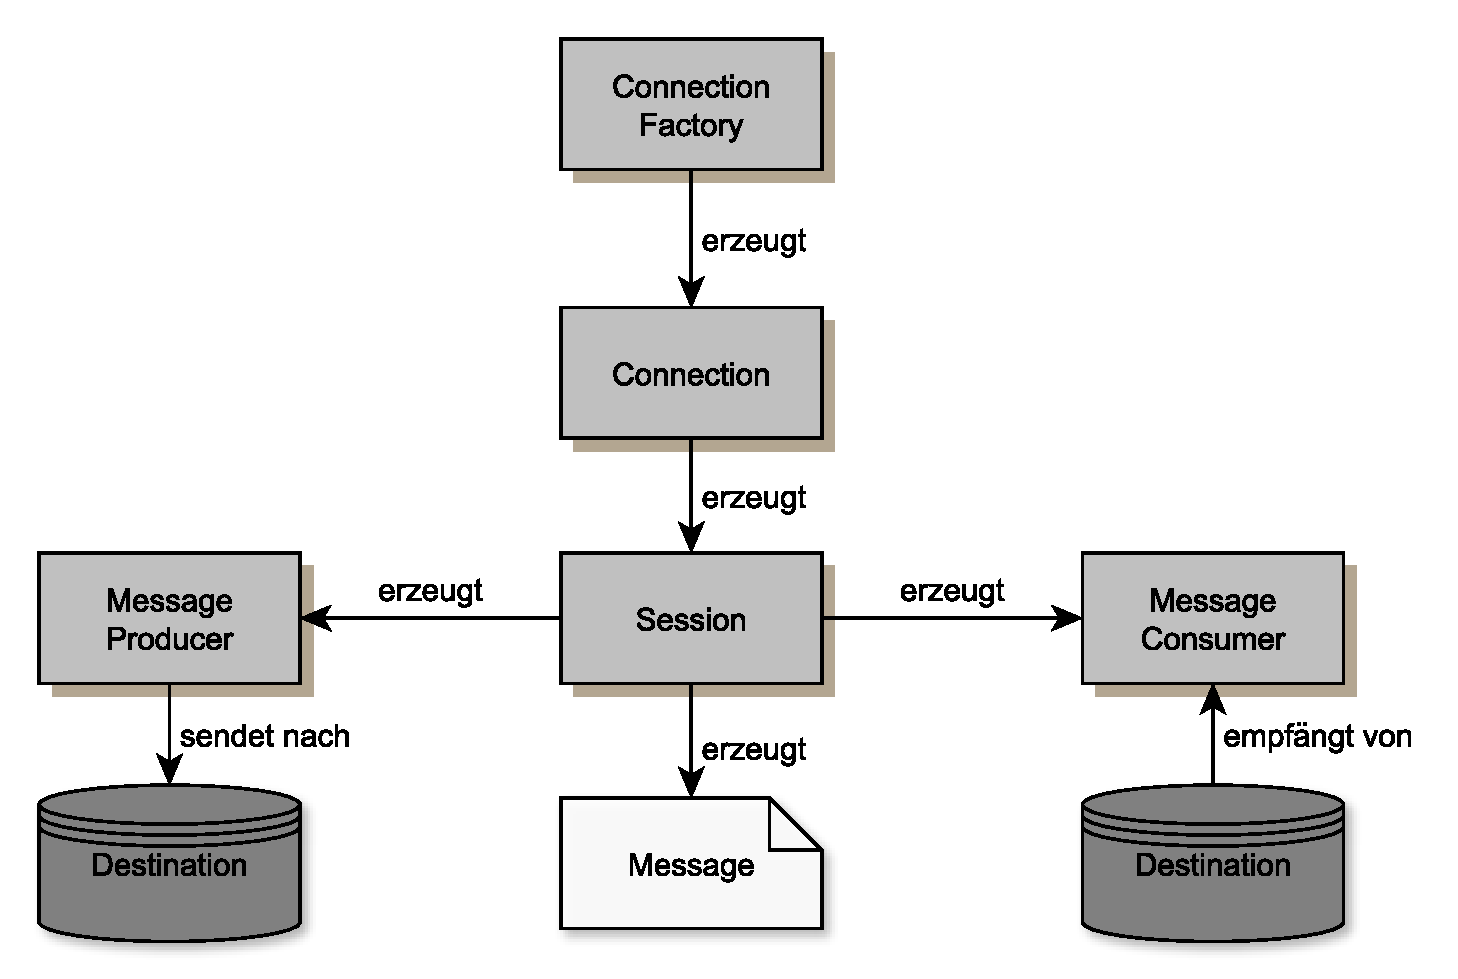
\includegraphics[
        width=0.8\textwidth,
        keepaspectratio=true,
        clip=true]
        {assets/images/jms_api_overview}
    \caption{JMS Programmiermodell - Original Bild: \url{http://docs.oracle.com/javaee/1.3/jms/tutorial/1_3_1-fcs/doc/images/Fig3.1.gif} (Zugriff: 2013-09-15)}
    \label{fig:jms_api_overview}
\end{figure}

Die Grundstruktur einer JMS-Anwendung besteht aus einem \emph{JMS Provider}, der die Schnittstellen von JMS implementiert. Dieser JMS-Provider wird auch als \emph{Message Oriented Middleware} (MOM) bezeichnet und kümmert sich auch darum, dass Nachrichten zuverlässig verschickt werden. Hinzu kommt ein JMS-Client von dem Nachrichten verschickt und empfangen werden, die Nachrichten selber, sowie sogenannte \emph{Administered Objects}. Diese Administered Objects bestehen aus vorkonfigurierten \emph{ConnectionFactory}s für das Erstellen von Verbindungen (\emph{Connection}) zwischen Client und Provider und \emph{Destination}s als Sende- und Empfangsendpunkte von Nachrichten. Die Administered Objects können im Client über das \emph{Java Naming and Directory} Interface (JNDI)\footnote{JNDI API:\url{http://www.oracle.com/technetwork/java/index-jsp-137536.html}} API abgefragt werden.

JMS unterstützt zwei Verbindungsarten zum Übertragen von Nachrichten: Queue- und Topic-basiert. Als Queue-basiert wird eine Punkt-zu-Punkt Verbindung bezeichnet. Hier werden Nachrichten nur zwischen zwei Clients übertragen und gegebenenfalls in einer Warteschlange zwischengespeichert. Hinter Topic-basiert verbirgt sich ein Publish-Subscribe-Mechanismus bei dem ein Client Nachrichten an eine Topic-Destination schickt und andere Clients sich auf dieses Topic anmelden können, um dann die Nachrichten des ersten Clients zu empfangen. Ob Queue oder Topic-basiert, wird über die Art der Destination ausgewählt.

Sollen nun Nachrichten von einem Client verschickt beziehungsweise empfangen werden, muss mit einer ConnectionFactory eine neue Connection zu einer MOM aufgebaut werden. Mit dieser Connection wird danach eine \emph{Session} erstellt, die als Kontext zum Senden und Empfangen verwendet wird. Für das versenden von Nachrichten muss mit dem Sessionobjekt ein \emph{MessageProducer} erstellt werden. Für das Empfangen entsprechend einen \emph{MessageConsumer}. Abbildung \ref{fig:jms_api_overview} zeig noch einmal den Zusammenhang aller JMS Komponenten.

\begin{lstlisting}[
    caption={JMS Beispiel}\label{lst:jms_beispiel},
    captionpos=t]
Context ctx = new InitialContext();
ConnectionFactory connectionFactory = (ConnectionFactory) ctx.lookup("ConnectionFactory");

Connection connection = connectionFactory.createConnection();
connection.start();

Session session = connection.createSession();
Destination destination = session.createTopic("topic-test");

MessageProducer msgProducer = session.createProducer(destination);
Message msg = session.createTextMessage("Hallo World!");
msgProducer.send(msg);
\end{lstlisting}

Listing \ref{lst:jms_beispiel} zeig ein kleines Beispiel zum Senden eine Textnachricht mit JMS. Die erste und zweite Zeile zeigt wie ein JNDI Kontext erstellt und nach einer vordefinierten ConnectionFactory mit den Name \enquote{ConnectionFactory} gesucht wird. Mit dieser ConnectionFactory wird dann eine neue Connection erstellt und gestartet. Danach folgt in Zeile 7 und 8 das Erstellen einer neuen Session und die Definition eins Topics mit dem Namen \enquote{topic-test} als Destination. In der zehnten Zeile wird dann der MessageProducer zum Senden von Nachrichten und in der Folgezeile die zu sendende Textnachricht erzeugt. Diese wird dann in der letzten Zeile vom MessageProducer an das Topic verschickt.

% subsection java_messaging_service (end)

\subsection{Enterprise Integration Patterns (EIP)} % (fold)
\label{sub:enterprise_integration_pattern}

Bezeichnungen wie \enquote{Iterator}, \enquote{Factory Method}, \enquote{Observer} oder \enquote{Proxy} hat bestimmt schon jeder Programmieren mindestens einmal gehört. Hierbei handelt es sich im sogenannte Entwurfsmuster für Softwareprogramme. Sie sind Schablonen für Lösungen von Problemen, die in der Entwicklung von Software immer wieder auftreten und sich als hilfreich erwiesen haben. Auch in der Integration von verschiedenen Geschäftsanwendungen in ein System treten solche Muster immer wieder auf. Gregor Hohpe und Bobby Woolf beschreiben in ihren Buch \enquote{Enterprise Integration Patterns: Designing, Building, and Deploying Messaging Solutions}\cite{Hohpe:2003:EIP:940308} eine Vielzahl solcher EIP für die Integration mit MOM. Alle hier aufzuzählen würde jedoch den Rahmen dieser Arbeit sprengen. Aus diesem Grund werden in Tabelle \ref{tbl:eip_beispiel_muster} fünf Muster inklusive der verwendeten Symbole vorgestellt, die später noch vorkommen werden. Die restlichen Muster sind auf der Webseite der EIP\footnote{\url{http://www.enterpriseintegrationpatterns.com/toc.html}} zu finden.

\begin{table}[ht]
    \centering
    \caption{Ausgewählte Beispiele von EIP}
    \begin{tabular}{c|c|p{9cm}}
        \textbf{Icon} & 
        \textbf{Name} & 
        \textbf{Beschreibung} \\ 
        \hline

        \raisebox{-0.7\totalheight}{
\includegraphics[
            width=1cm,
            keepaspectratio=true]
        {assets/images/eip/message_alt}} & 
        \emph{Message} & 
        Über Nachrichten werden Daten zwischen zwei oder mehr Systemen ausgetauscht. \\

        \raisebox{-0.7\totalheight}{
\includegraphics[
                width=3cm,
                keepaspectratio=true]
            {assets/images/eip/channel}}& 
        \emph{Channel} &
        Ein Channel beschreibt einen Nachrichtenkanal, über den Nachrichten von einem System in ein anderes verschickt werden können.\\

        \raisebox{-0.7\totalheight}{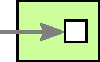
\includegraphics[
                width=3cm,
                keepaspectratio=true]
            {assets/images/eip/endpoint}}& 
        \emph{Endpoint} & 
        Endpoints sind Schnittstellen in einem System, von dem Nachrichten in einen Kanal gesendet oder von dort Empfangen werden. \\
        &&\\


        \raisebox{-0.7\totalheight}{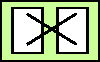
\includegraphics[
                width=3cm,
                keepaspectratio=true]
            {assets/images/eip/message_translator}} & 
        \emph{Message Translator} & 
        Nicht immer liegt eine Nachricht im richtigen Format für ein System vor. Durch Message Translators können diese in das gewünschte Format konvertiert werden.\\

        \raisebox{-0.7\totalheight}{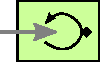
\includegraphics[
                width=3cm,
                keepaspectratio=true]
            {assets/images/eip/polling_consumer}} &
        \emph{Polling Consumer} &
        Manchmal möchte ein Programm Nachrichten nicht verarbeiten wenn sie ankommen, sondern dann wenn es bereit dazu ist. Ein PollingConsumer fragt also erst zu bestimmten Zeitpunkten ab, ob Nachrichten für ihn vorliegen. 
    \end{tabular}
    \label{tbl:eip_beispiel_muster}
\end{table}

\pagebreak

\subsubsection{Apache Camel} % (fold)
\label{ssub:apache_camel}

\emph{Apache Camel}\cite{ApacheCamel} (kurz: Camel) ist ein Projekt der Apache Software Foundation (kurz: Apache) für das Routen und Verteilen von Nachrichten zur Integration von System auf Basis von definierten Regeln. Camel stellt dazu eine Java-basierte API für den Einsatz der EIP bereit. Die Regeln für die Routen, die Nachrichten nehmen können, können direkt in Java, aber auch durch das Spring Framework\footnote{\url{http://www.springsource.org/}} in XML definiert werden. 

\begin{lstlisting}[
    caption={Apache Camel Beispiel}\label{lst:camel_beispiel},
    captionpos=t]
RouteDefinition rd = new RouteDefinition()
    .from('timer://helloTimer?period=3000')
    .to('log:helloLog');

CamelContext camelContext = new DefaultCamelContext();
camelContext.addRouteDefinition( rd );
camelContext.start();
\end{lstlisting}

Listing \ref{lst:camel_beispiel} zeig ein Beispiel, wie eine Nachrichtenroute in Java für Camel definiert werden kann. In der ersten Zeile wird über die Klasse \texttt{RouteDefinition} eine neue Route erstellt. Über die Methode \texttt{from(\dots)} wird der Endpunkt, vom dem die Route ausgeht, festgelegt. Welcher Endpunkt das genau seien soll, kann auf zwei Arten definiert werden. Man übergibt der Methode direkt ein Objekt einer Klasse die das Interface \texttt{Endpoint} implementiert oder man macht es, wie hier im Beispiel, über eine URI. Diese URI baut sich auf folgende Weise zusammen: Der Teil bis zum Doppelpunkt, das sogenannte \enquote{Schema}, legt die Komponente (engl. \texttt{Component}) fest, von der ein Endpunkt erzeugen werden soll. In diesem Falls ist es eine Timer-Komponente, deren Endpunkt im periodischen Abstand Event-Nachrichten verschickt. Der Rest der URI wird zur Konfiguration an den Endpunkt übergeben. \enquote{helloTimer} steht hier für einen Namen für den Timer und der Parameter \enquote{period} gibt den zeitlichen Abstand zwischen zwei Event-Nachrichten an. Das Ziel der Route wird mit der Methode \texttt{to(\dots)} in Zeile 3 festgelegt. Für das Ziel wird hier eine Log-Komponente mit dem Namen \enquote{helloLog} festgelegt, die alle reinkommenden Nachrichten protokolliert. In der fünften Zeile wird ein \texttt{CamelContext} Objekt, das für die Verwaltung und Ausführung der Routen verantwortliche ist, erstellt. Die Route wird dann dem CamelContext hinzugefügt und die Ausführung in der letzten Zeile gestartet. Nun wird der Timer alle 3000 Millisekunden eine neue Event-Nachricht erzeugen und an den CamelContext schicken. Dieser leitet die Nachricht dann an das durch die Route definierte Ziel und wird dort von der Log-Komponente ausgeben.

Für Camel existieren eine Menge vorgefertigter Komponenten\footnote{\url{http://camel.apache.org/components.html}} die ein großes Spektrum an Anwendungsmöglichkeiten abdeckt. Es gibt Komponenten für die Anbindung an HTTP-Webserver, JMS-Provider, E-Mail-Server, RSS/Atom-Feeds\footnote{\url{http://www.rssboard.org/rss-specification}} und viele mehr. 

% subsubsection apache_camel (end)

% subsection enterprise_integration_patternl (end)

% section datenverteilung (end)

\section{Lernplattformen und soziale Online-Netzwerke} % (fold)
\label{sec:lernplattformen_und_soziale_online_netzwerke}

An dieser Stelle sollen kurz einige Lernplattformen und soziale Online-Netzwerke vorgestellt werden, die im späteren Verlauf dieser Arbeit für die Implementierung verwendet wurden. Im Einzelnen waren dies \emph{Moodle}, \emph{Canvas}, \emph{Facebook}, \emph{Google+} und \emph{Youtube}, da sie einen guten Schnitt von den Plattformen bilden, die heutzutage sowohl im Bereich E-Learning als auch von der breiten Masse verwendet werden.

\subsection{Moodle} % (fold)
\label{sub:moodle}
%% korrigiert am 2013-10-01

Moodle\footnote{\url{https://moodle.org/}} ist ein weit verbreitetes LMS. Die Hauptaufgabe liegt im Verwalten von Online-Kursen im Bereich E-Learning. Hierzu bietet Moodle von Haus aus eine große Menge an Funktionen für die Verwaltung des Kurses und die Kommunikation zwischen Lehrenden und Lernenden. Es bietet die Möglichkeit Aufgaben an die Teilnehmer zu verteilen, Fragebögen zu erstellen, zusätzlichen Kursmaterialien bereitzustellen und den Lernerfolg durch Benotung und Feedback zu kontrollieren. Funktionen für die Unterstützung des kollaborativen Lernens sind ebenfalls vorhanden. Teilnehmer können Lerngruppen bilden, sich über persönliche Nachrichten austauschen, gemeinsam an Wikis arbeiten oder in Foren diskutieren. 
% \begin{figure}[ht]
%     \centering
%     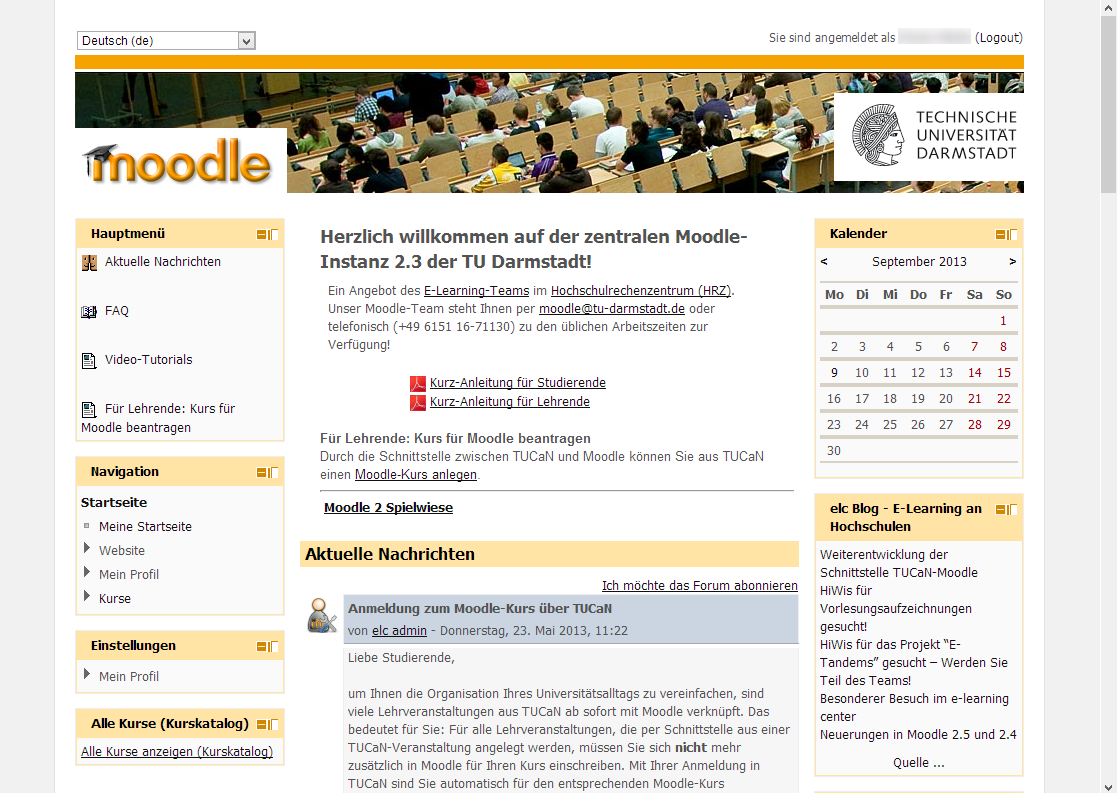
\includegraphics[
%         width=0.7\textwidth,
%         keepaspectratio=true,
%     ]{assets/images/tud_moodle_screenshot}
%     \caption{Moodleinstanz der TU Darmstadt}
%     \label{fig:moodle_tud}
% \end{figure}

Moodle wurde in der Programmiersprache PHP geschrieben und unterstützt die  Datenbanken MySQL, PostgrSQL, MSSQL und Oracle. Die Installation von weiteren Funktionalitäten ist durch von Dritten geschriebenen Erweiterungen möglich. Seit Version 2.0 können für Moodle auch Webservices installiert werden. So ist es auch externe Anwendungen erlaubt auf interne Funktionen und Daten zugreifen.

% subsection moodle (end)

\subsection{Canvas} % (fold)
\label{sub:canvas}

Das von der Firma Instructure\footnote{\url{https://www.instructure.com}} entwickelte \emph{Canvas} ist ein recht neues, unter Open Source Lizenz gestelltes LMS. Vom Funktionsumfang ist es Moodle nicht unähnlich. Es existiert eine Verwaltung einzelner Kurse. Innerhalb dieser Kurse können in einem Forum Diskussionen geführt und Lernmieteralien hoch- und heruntergeladenen werden. Verteilung von Aufgaben, deren Benotung und ein Benachrichtigungssystem existiert ebenfalls. Canvas erlaubt auch das Einbinden von externen Diensten zum kollaborativen Lernen und Arbeiten wie Google Docs\footnote{\url{https://drive.google.com}} oder der Webkonferenz Anwendung BigBlueButton\footnote{\url{http://www.bigbluebutton.org}}.

% \begin{figure}[ht]
%     \centering
%     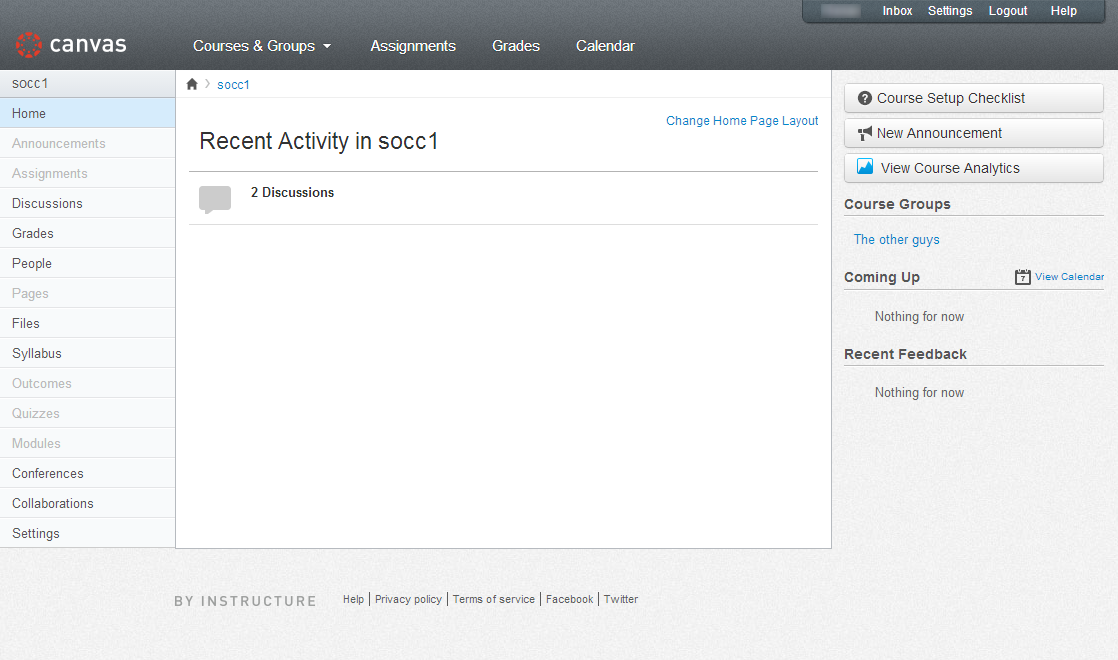
\includegraphics[
%         width=0.7\textwidth,
%         keepaspectratio=true,
%     ]{assets/images/canvas_lms}
%     \caption{Instructure Canvas}
%     \label{fig:canvas_lms}
% \end{figure}

Canvas wird mit dem Webframework \emph{Ruby on Rails}\footnote{\url{http://rubyonrails.org}} entwickelt. Eine Erweiterung der Funktionalität von Canvas ist durch das einbinden von Programmen möglich, die den \emph{Learning Tools Interoperability™} (LTI) Standard erfüllen. Einige solcher Programme finden sich auf der Webseite \url{https://www.edu-apps.org}. Unter anderem Programme zum Suchen und Einbinden von Youtube Videos, Wikipedia Artikeln, GitHub Gists\footnote{\url{https://gist.github.com}} und vielen weiteren.

% subsection canvas (end)

\subsection{Facebook} % (fold)
\label{sub:facebook}
%% korrigiert am 2013-10-01

Das soziale Online-Netzwerk Facebook\footnote{\url{https://www.facebook.com/}} kann mit rund 699 Millionen aktiven Benutzern täglich zu den aktuell beliebtesten Vertreter seiner Art bezeichnet werden (siehe \cite{Facebook2013}). Facebook erlaubt es, wie alle sozialen Online-Netzwerke, bekannte Personen in Freundeslisten zusammenzufassen und mit ihnen private Nachrichten auszutauschen. Beiträge wie Texte, Fotos oder Videos können auf einer Art Pinnwand, der \enquote{Wall}, öffentlich oder nur mit Freunden geteilt werden. Benutzer mit gemeinsamen Interessen können dazu eigene Gruppen bilden und dort auf einer eigen Wall Beiträge veröffentlichen oder die anderer kommentieren. Wie in der Einleitung schon erklärt, zeigt Qiyun Wang et. al. \cite{Wang2012} das sich Facebook, wenn auch mit Einschränkungen, wunderbar zur Verwaltung und Nutzung durch Kurse und Lerngruppen eignet. Die gleiche Erfahrung teilte Anthony Fontana \cite{Fontana2009,FacebookinEducarion2010}, der Facebook als Alternative zum bestehenden System der Bowling Green State University in Ohio, USA verwendete.

% subsection facebook (end)

\subsection{Google+} % (fold)
\label{sub:google_plus}
%% korrigiert am 2013-10-01

Google+\footnote{https://plus.google.com} ist ein 2011 von Google gestartetes soziales Online-Netzwerk. Seit Anfang 2013 ist Google+, von der Anzahl der aktiven Benutzer her gesehen, auf Platz 2 hinter Marktführer Facebook (siehe \cite{Thomas2013}). Vom Funktionsumfang sind sich beide sehr ähnlich. Auf Google+ können andere Benutzer in sogenannten \enquote{Circles} sortiert werden, welche den auf Facebook genutzten Freundeslisten entspricht. Jeder Benutzer hat einen eigenen \enquote{Activity Stream} in dem er Beiträge (Activity) öffentlich oder nur für ein oder mehrere Circles verfassen kann. Das Gründen von Gruppen für bestimmte Interessensbereiche ist auch in Google+ möglich und werden dort als \enquote{Community} bezeichnet.

% subsection google_ (end)

\subsection{Youtube} % (fold)
\label{sub:youtube}

Youtube\footnote{\url{https://www.youtube.com}} gehört wohl heute zu den beliebtesten Anlaufpunkten im Internet, wenn es um das Thema Videos geht. Monatlich nutzen über 1 Milliarde Nutzer die Seite und pro Minute werden 100 Stunden neuer Videos hochgeladen (siehe \cite{youtube2013statistics}). Doch nicht das komplette Videomaterial besteht aus Katzen, Musik oder Unfallvideos. Ein Teil der Benutzer, die eigene Videos hochladen, wollen anderen Dinge beibringen, weil es in ihr Interessengebiet passt oder früher selber Probleme damit hatten. Einer erklärt die Logarithmengesetze, ein anderer wie man Feuer ohne Feuerzeug macht und eine ganz andere gibt Schönheitstipps. Youtube ist also auch im E-Learning Bereich gut einsetzbar. Lehrende können eigene Videos hochladen, von anderen interessante Videos in Playlisten zusammenfassen und die Lernenden können über Kommentare Fragen zum Inhalt stellen. 

% subsection youtube (end)

% section lernplattformen_und_soziale_online_netzwerke (end)

\section{Verwandte Arbeiten und Projekte} % (fold)
\label{sec:verwandte_arbeiten_und_projekte}

Leider gibt es so gut wie kein Projekt, dass sich direkt mit den Austausch von Diskussionsbeiträgen zwischen unterschiedlichen Plattformen befasst. Eines dieser doch existierenden Projekte wurde weiter oben mit SIOC in Verbindung mit FOAF schon vorgestellt. Nichtsdestotrotz existieren Arbeiten und Projekte die sich damit befassen, wie jeder seine Daten, die er irgendwann und irgendwo in einen sozialen Online-Netzwerk hinterlassen hat, wieder zurück unter seine Kontrolle bringt. Von diesem Punkt ist es nicht mehr weit, diese Daten wieder in eine andere Plattform zu übertragen, falls dies gewünscht ist.  
%\todo[inline]{Verwandte Arbeiten Einleitung schreiben}

\subsection{What happens when Facebook is gone?} % (fold)
\label{sub:what_happens_when_facebook_is_gone}

Frank McCown und Michael L. Nelson beschreiben in ihrem Bericht \enquote{What happens when Facebook is gone?}\cite{McCown2009}, wie Möglichkeiten aussehen können, die unsere Daten von sozialen Online-Netzwerken (hier im speziellen Fall von Facebook) für uns und die Nachwelt archivieren können. Zum Beispiel, wenn eine Person einen großen Teil seines persönlichen Lebens auf Facebook verbringt und plötzlich stirbt. Wie sollen seine Angehörigen an nicht öffentliche Texte, Bilder, Videos heran kommen, wenn sie in der Regel keinen Zugriff auf das Benutzerkonto haben, da der Verstorbene so etwas nicht vorhersehen konnte. Oder wenn ein Benutzer mit seinen Daten in ein anderes soziales Online-Netzwerk umziehen will, sei dies bei Facebook (zum damaligen Zeitpunkt) nur schwer möglich.

\begin{quote}
    \enquote{It is also likely he was not prepared to die at such a young age, and much of his personal life, which lies in the digital \grqq cloud\grqq, may never be accessible to his loved ones}
    \cite[S.\,251]{McCown2009}
\end{quote}

Zum Anlegen eines solchen Archivs wurden mehrere Ansätze vorgestellt. Die einfachste Ansatz wäre die E-Mail-Benachrichtigung zu aktivieren und alle neuen Beiträge in einem E-Mail-Postfach zu sichern. So können aber nur alle neuen Beiträge erfasst werden. Alte bleiben weiterhin in Facebook. Eine sehr aufwändige Möglichkeit wäre es Bildschirmfotos von den Beiträgen zu machen und diese durch ein Texterkennungsprogramm laufen zu lassen. Die dadurch erzeugten Dateien können dann in einer Datenbank gespeichert werden. Heutige Internetbrowser bieten es zusätzlich zum Anzeigen von Webseite auch das Herunterladen selbiger an. Dabei wird die HTML-Datei inklusive aller darin enthaltenen weiteren Dateien wie Bilder, Videos und CSS-Dateien gespeichert. Die so archivierte Seite hat dann im beschränkten Umfang genau das gleiche Aussehen und Verhalten wie die original Seite. Ebenfalls wäre eine Nutzung der von Facebook bereitgestellten API für Anwendungen eine Überlegung wert. 2009 war diese API noch sehr eingeschränkt. Gerade der Zugriff auf Beiträge und private Nachrichten war nicht möglich (siehe \cite[S.\,253, Table 1]{McCown2009}). Für die Implementierung eines Beispiel Programms wurde ein fünfter Ansatz gewählt. Über einen sogenannten Webcrawler oder eine Erweiterung für den Browser werden relevante Seiten automatisch heruntergeladen und in einen Archiv abgelegt. Dynamische Inhalte sollen kein Problem darstellen, da die Seite erst heruntergeladen wird, wenn alle Aufrufe dynamischer Funktionen abgeschlossen ist. Die archivierten Dateien können dann mittels Techniken des Datamining verarbeitet und als Atom/RSS-Feed bereitgestellt werden. 

% subsection what_happens_when_facebook_is_gone_ (end)

\subsection{Reclaim Social} % (fold)
\label{sub:reclaim_social}

Ein Problem bei der heutigen Landschaft an sozialen Online-Netzwerken ist die Tatsache, dass man nicht nur ein einziges für alles benutzt, sondern mehrere gleichzeitig. Einige davon fast täglich, andere werden immer weniger genutzt und irgendwann vergessen. Zugleich ist alles was man dort geschrieben oder hochgeladen hat auf den Server der Betreiber \enquote{gefangen}. Genau aus diesem Grund haben Sascha Lobo und Felix Schwenzel auf der Netzkonferenz re:publica\footnote{\url{http://re-publica.de/}} 2013 ihr Projekt \emph{Reclaim Social} \cite{Schwenzel2013} vorgestellt.

Ziel dieses Projektes ist es von einem selber erzeugten Daten aus allen möglichen Quellen auf seinen eigenen Blog zu spiegeln und so einen zentrale Anlaufstelle für seine eigenen Inhalte schaffen. Reclaim Social baut dazu auf der weit verbreiteten Blogsoftware \emph{WordPress\footnote{\url{http://wordpress.org/}}} und der dafür vorhandenen Erweiterung \emph{FeedWordPress}\footnote{\url{http://feedwordpress.radgeek.com/}} auf. Diese Kombination ermöglichst alle Internetseiten, welche einen RSS/Atom-Feed anbieten, in die Datenbank von WordPress zu überführen. Das Problem hierbei besteht darin, dass sehr beliebte Internetseiten solche RSS/Atom-Feeds nicht anbieten (Facebook, Google+). Für einige solcher Seiten wurden \enquote{proxy-scripte}\cite[\enquote{Tech Specs Details}]{Schwenzel2013} implementiert, welche für diese einen RSS-Feed emulieren. Zugleich können in den Feeds enthaltende Medien, wie Bilder und Videos (bisher nur als Referenz), heruntergeladen und in WordPress gespeichert werden. So ist es möglich alle gespiegelten Daten einfach zu durchsuchen oder nach bestimmten Kriterien zu filtern. Zusätzlich können alle Freunde, welche auch Reclaim Social einsetzen, in einen Kontaktliste eingetragen und so auch deren Inhalte eingebunden werden.

Aktuell befindet sich dieses Projekt noch im Alphastadium und die Installation ist relativ kompliziert. Es ist aber geplant eine eigene Erweiterung für WordPress zu schreiben \enquote{The goal is to build just one Reclaim Social-plugin for any wordpress user}\cite[\enquote{How Does It Work}]{Schwenzel2013}

% subsection reclaim_social (end)

% section verwandte_arbeiten_und_projekte (end)

% chapter grundlagen (end)